% REV01 Sun 27 Jun 2021 07:29:17 WIB
% START Tue 04 May 2021 13:55:16 WIB

\chapter{SETTING TRAPS}

Plashwater Weir Mill Lock looked tranquil and pretty on an evening in
the summer time. A soft air stirred the leaves of the fresh green trees,
and passed like a smooth shadow over the river, and like a smoother
shadow over the yielding grass. The voice of the falling water, like
the voices of the sea and the wind, were as an outer memory to a
contemplative listener; but not particularly so to Mr Riderhood, who sat
on one of the blunt wooden levers of his lock-gates, dozing. Wine must
be got into a butt by some agency before it can be drawn out; and the
wine of sentiment never having been got into Mr Riderhood by any agency,
nothing in nature tapped him.

As the Rogue sat, ever and again nodding himself off his balance, his
recovery was always attended by an angry stare and growl, as if, in the
absence of any one else, he had aggressive inclinations towards himself.
In one of these starts the cry of ‘Lock, ho! Lock!’ prevented his
relapse into a doze. Shaking himself as he got up like the surly brute
he was, he gave his growl a responsive twist at the end, and turned his
face down-stream to see who hailed.

It was an amateur-sculler, well up to his work though taking it easily,
in so light a boat that the Rogue remarked: ‘A little less on you, and
you’d a’most ha’ been a Wagerbut’; then went to work at his windlass
handles and sluices, to let the sculler in. As the latter stood in his
boat, holding on by the boat-hook to the woodwork at the lock side,
waiting for the gates to open, Rogue Riderhood recognized his ‘T’other
governor,’ Mr Eugene Wrayburn; who was, however, too indifferent or too
much engaged to recognize him.

The creaking lock-gates opened slowly, and the light boat passed in as
soon as there was room enough, and the creaking lock-gates closed upon
it, and it floated low down in the dock between the two sets of gates,
until the water should rise and the second gates should open and let it
out. When Riderhood had run to his second windlass and turned it, and
while he leaned against the lever of that gate to help it to swing
open presently, he noticed, lying to rest under the green hedge by the
towing-path astern of the Lock, a Bargeman.

The water rose and rose as the sluice poured in, dispersing the scum
which had formed behind the lumbering gates, and sending the boat up,
so that the sculler gradually rose like an apparition against the light
from the bargeman’s point of view. Riderhood observed that the bargeman
rose too, leaning on his arm, and seemed to have his eyes fastened on
the rising figure.

But, there was the toll to be taken, as the gates were now complaining
and opening. The T’other governor tossed it ashore, twisted in a piece
of paper, and as he did so, knew his man.

‘Ay, ay? It’s you, is it, honest friend?’ said Eugene, seating himself
preparatory to resuming his sculls. ‘You got the place, then?’

‘I got the place, and no thanks to you for it, nor yet none to Lawyer
Lightwood,’ gruffly answered Riderhood.

‘We saved our recommendation, honest fellow,’ said Eugene, ‘for the next
candidate--the one who will offer himself when you are transported or
hanged. Don’t be long about it; will you be so good?’

So imperturbable was the air with which he gravely bent to his work that
Riderhood remained staring at him, without having found a retort, until
he had rowed past a line of wooden objects by the weir, which showed
like huge teetotums standing at rest in the water, and was almost hidden
by the drooping boughs on the left bank, as he rowed away, keeping
out of the opposing current. It being then too late to retort with
any effect--if that could ever have been done--the honest man confined
himself to cursing and growling in a grim under-tone. Having then
got his gates shut, he crossed back by his plank lock-bridge to the
towing-path side of the river.

If, in so doing, he took another glance at the bargeman, he did it by
stealth. He cast himself on the grass by the Lock side, in an indolent
way, with his back in that direction, and, having gathered a few blades,
fell to chewing them. The dip of Eugene Wrayburn’s sculls had become
hardly audible in his ears when the bargeman passed him, putting the
utmost width that he could between them, and keeping under the hedge.
Then, Riderhood sat up and took a long look at his figure, and then
cried: ‘Hi--I--i! Lock, ho! Lock! Plashwater Weir Mill Lock!’

The bargeman stopped, and looked back.

‘Plashwater Weir Mill Lock, T’otherest gov--er--nor--or--or--or!’ cried
Mr Riderhood, with his hands to his mouth.

The bargeman turned back. Approaching nearer and nearer, the bargeman
became Bradley Headstone, in rough water-side second-hand clothing.

‘Wish I may die,’ said Riderhood, smiting his right leg, and laughing,
as he sat on the grass, ‘if you ain’t ha’ been a imitating me,
T’otherest governor! Never thought myself so good-looking afore!’

Truly, Bradley Headstone had taken careful note of the honest man’s
dress in the course of that night-walk they had had together. He must
have committed it to memory, and slowly got it by heart. It was
exactly reproduced in the dress he now wore. And whereas, in his own
schoolmaster clothes, he usually looked as if they were the clothes of
some other man, he now looked, in the clothes of some other man or men,
as if they were his own.

‘THIS your Lock?’ said Bradley, whose surprise had a genuine air; ‘they
told me, where I last inquired, it was the third I should come to. This
is only the second.’

‘It’s my belief, governor,’ returned Riderhood, with a wink and shake of
his head, ‘that you’ve dropped one in your counting. It ain’t Locks as
YOU’VE been giving your mind to. No, no!’

As he expressively jerked his pointing finger in the direction the boat
had taken, a flush of impatience mounted into Bradley’s face, and he
looked anxiously up the river.

‘It ain’t Locks as YOU’VE been a reckoning up,’ said Riderhood, when the
schoolmaster’s eyes came back again. ‘No, no!’

‘What other calculations do you suppose I have been occupied with?
Mathematics?’

‘I never heerd it called that. It’s a long word for it. Hows’ever,
p’raps you call it so,’ said Riderhood, stubbornly chewing his grass.

‘It. What?’

‘I’ll say them, instead of it, if you like,’ was the coolly growled
reply. ‘It’s safer talk too.’

‘What do you mean that I should understand by them?’

‘Spites, affronts, offences giv’ and took, deadly aggrawations, such
like,’ answered Riderhood.

Do what Bradley Headstone would, he could not keep that former flush of
impatience out of his face, or so master his eyes as to prevent their
again looking anxiously up the river.

‘Ha ha! Don’t be afeerd, T’otherest,’ said Riderhood. ‘The T’other’s got
to make way agin the stream, and he takes it easy. You can soon come up
with him. But wot’s the good of saying that to you! YOU know how fur
you could have outwalked him betwixt anywheres about where he lost the
tide--say Richmond--and this, if you had a mind to it.’

‘You think I have been following him?’ said Bradley.

‘I KNOW you have,’ said Riderhood.

‘Well! I have, I have,’ Bradley admitted. ‘But,’ with another anxious
look up the river, ‘he may land.’

‘Easy you! He won’t be lost if he does land,’ said Riderhood. ‘He must
leave his boat behind him. He can’t make a bundle or a parcel on it, and
carry it ashore with him under his arm.’

‘He was speaking to you just now,’ said Bradley, kneeling on one knee on
the grass beside the Lock-keeper. ‘What did he say?’

‘Cheek,’ said Riderhood.

‘What?’

‘Cheek,’ repeated Riderhood, with an angry oath; ‘cheek is what he said.
He can’t say nothing but cheek. I’d ha’ liked to plump down aboard of
him, neck and crop, with a heavy jump, and sunk him.’

Bradley turned away his haggard face for a few moments, and then said,
tearing up a tuft of grass:

‘Damn him!’

‘Hooroar!’ cried Riderhood. ‘Does you credit! Hooroar! I cry chorus to
the T’otherest.’

‘What turn,’ said Bradley, with an effort at self-repression that forced
him to wipe his face, ‘did his insolence take to-day?’

‘It took the turn,’ answered Riderhood, with sullen ferocity, ‘of hoping
as I was getting ready to be hanged.’

‘Let him look to that,’ cried Bradley. ‘Let him look to that! It will
be bad for him when men he has injured, and at whom he has jeered, are
thinking of getting hanged. Let HIM get ready for HIS fate, when that
comes about. There was more meaning in what he said than he knew of, or
he wouldn’t have had brains enough to say it. Let him look to it; let
him look to it! When men he has wronged, and on whom he has bestowed
his insolence, are getting ready to be hanged, there is a death-bell
ringing. And not for them.’

Riderhood, looking fixedly at him, gradually arose from his recumbent
posture while the schoolmaster said these words with the utmost
concentration of rage and hatred. So, when the words were all spoken,
he too kneeled on one knee on the grass, and the two men looked at one
another.

‘Oh!’ said Riderhood, very deliberately spitting out the grass he had
been chewing. ‘Then, I make out, T’otherest, as he is a-going to her?’

‘He left London,’ answered Bradley, ‘yesterday. I have hardly a doubt,
this time, that at last he is going to her.’

‘You ain’t sure, then?’

‘I am as sure here,’ said Bradley, with a clutch at the breast of his
coarse shirt, ‘as if it was written there;’ with a blow or a stab at the
sky.

‘Ah! But judging from the looks on you,’ retorted Riderhood, completely
ridding himself of his grass, and drawing his sleeve across his mouth,
‘you’ve made ekally sure afore, and have got disapinted. It has told
upon you.’

‘Listen,’ said Bradley, in a low voice, bending forward to lay his hand
upon the Lock-keeper’s shoulder. ‘These are my holidays.’

‘Are they, by George!’ muttered Riderhood, with his eyes on the
passion-wasted face. ‘Your working days must be stiff ‘uns, if these is
your holidays.’

‘And I have never left him,’ pursued Bradley, waving the interruption
aside with an impatient hand, ‘since they began. And I never will leave
him now, till I have seen him with her.’

‘And when you have seen him with her?’ said Riderhood.

‘--I’ll come back to you.’

Riderhood stiffened the knee on which he had been resting, got up, and
looked gloomily at his new friend. After a few moments they walked side
by side in the direction the boat had taken, as if by tacit consent;
Bradley pressing forward, and Riderhood holding back; Bradley getting
out his neat prim purse into his hand (a present made him by penny
subscription among his pupils); and Riderhood, unfolding his arms to
smear his coat-cuff across his mouth with a thoughtful air.

‘I have a pound for you,’ said Bradley.

‘You’ve two,’ said Riderhood.

Bradley held a sovereign between his fingers. Slouching at his side with
his eyes upon the towing-path, Riderhood held his left hand open, with
a certain slight drawing action towards himself. Bradley dipped in his
purse for another sovereign, and two chinked in Riderhood’s hand, the
drawing action of which, promptly strengthening, drew them home to his
pocket.

‘Now, I must follow him,’ said Bradley Headstone. ‘He takes this
river-road--the fool!--to confuse observation, or divert attention, if
not solely to baffle me. But he must have the power of making himself
invisible before he can shake Me off.’

Riderhood stopped. ‘If you don’t get disapinted agin, T’otherest, maybe
you’ll put up at the Lock-house when you come back?’

‘I will.’

Riderhood nodded, and the figure of the bargeman went its way along the
soft turf by the side of the towing-path, keeping near the hedge and
moving quickly. They had turned a point from which a long stretch of
river was visible. A stranger to the scene might have been certain that
here and there along the line of hedge a figure stood, watching the
bargeman, and waiting for him to come up. So he himself had often
believed at first, until his eyes became used to the posts, bearing the
dagger that slew Wat Tyler, in the City of London shield.

Within Mr Riderhood’s knowledge all daggers were as one. Even to Bradley
Headstone, who could have told to the letter without book all about Wat
Tyler, Lord Mayor Walworth, and the King, that it is dutiful for youth
to know, there was but one subject living in the world for every sharp
destructive instrument that summer evening. So, Riderhood looking after
him as he went, and he with his furtive hand laid upon the dagger as he
passed it, and his eyes upon the boat, were much upon a par.

The boat went on, under the arching trees, and over their tranquil
shadows in the water. The bargeman skulking on the opposite bank of the
stream, went on after it. Sparkles of light showed Riderhood when
and where the rower dipped his blades, until, even as he stood idly
watching, the sun went down and the landscape was dyed red. And then the
red had the appearance of fading out of it and mounting up to Heaven, as
we say that blood, guiltily shed, does.

Turning back towards his Lock (he had not gone out of view of it), the
Rogue pondered as deeply as it was within the contracted power of such
a fellow to do. ‘Why did he copy my clothes? He could have looked like
what he wanted to look like, without that.’ This was the subject-matter
in his thoughts; in which, too, there came lumbering up, by times, like
any half floating and half sinking rubbish in the river, the question,
Was it done by accident? The setting of a trap for finding out whether
it was accidentally done, soon superseded, as a practical piece of
cunning, the abstruser inquiry why otherwise it was done. And he devised
a means.

Rogue Riderhood went into his Lock-house, and brought forth, into the
now sober grey light, his chest of clothes. Sitting on the grass beside
it, he turned out, one by one, the articles it contained, until he came
to a conspicuous bright red neckerchief stained black here and there by
wear. It arrested his attention, and he sat pausing over it, until he
took off the rusty colourless wisp that he wore round his throat, and
substituted the red neckerchief, leaving the long ends flowing. ‘Now,’
said the Rogue, ‘if arter he sees me in this neckhankecher, I see him in
a sim’lar neckhankecher, it won’t be accident!’ Elated by his device, he
carried his chest in again and went to supper.

‘Lock ho! Lock!’ It was a light night, and a barge coming down summoned
him out of a long doze. In due course he had let the barge through
and was alone again, looking to the closing of his gates, when Bradley
Headstone appeared before him, standing on the brink of the Lock.

‘Halloa!’ said Riderhood. ‘Back a’ ready, T’otherest?’

‘He has put up for the night, at an Angler’s Inn,’ was the fatigued and
hoarse reply. ‘He goes on, up the river, at six in the morning. I have
come back for a couple of hours’ rest.’

‘You want ‘em,’ said Riderhood, making towards the schoolmaster by his
plank bridge.

‘I don’t want them,’ returned Bradley, irritably, ‘because I would
rather not have them, but would much prefer to follow him all night.
However, if he won’t lead, I can’t follow. I have been waiting about,
until I could discover, for a certainty, at what time he starts; if I
couldn’t have made sure of it, I should have stayed there.--This would
be a bad pit for a man to be flung into with his hands tied. These
slippery smooth walls would give him no chance. And I suppose those
gates would suck him down?’

‘Suck him down, or swaller him up, he wouldn’t get out,’ said Riderhood.
‘Not even, if his hands warn’t tied, he wouldn’t. Shut him in at both
ends, and I’d give him a pint o’ old ale ever to come up to me standing
here.’

Bradley looked down with a ghastly relish. ‘You run about the brink, and
run across it, in this uncertain light, on a few inches width of rotten
wood,’ said he. ‘I wonder you have no thought of being drowned.’

‘I can’t be!’ said Riderhood.

‘You can’t be drowned?’

‘No!’ said Riderhood, shaking his head with an air of thorough
conviction, ‘it’s well known. I’ve been brought out o’ drowning, and I
can’t be drowned. I wouldn’t have that there busted B’lowbridger aware
on it, or her people might make it tell agin’ the damages I mean to get.
But it’s well known to water-side characters like myself, that him as
has been brought out o drowning, can never be drowned.’

Bradley smiled sourly at the ignorance he would have corrected in one of
his pupils, and continued to look down into the water, as if the place
had a gloomy fascination for him.

‘You seem to like it,’ said Riderhood.

He took no notice, but stood looking down, as if he had not heard the
words. There was a very dark expression on his face; an expression
that the Rogue found it hard to understand. It was fierce, and full
of purpose; but the purpose might have been as much against himself as
against another. If he had stepped back for a spring, taken a leap, and
thrown himself in, it would have been no surprising sequel to the look.
Perhaps his troubled soul, set upon some violence, did hover for the
moment between that violence and another.

‘Didn’t you say,’ asked Riderhood, after watching him for a while with
a sidelong glance, ‘as you had come back for a couple o’ hours’ rest?’
But, even then he had to jog him with his elbow before he answered.

‘Eh? Yes.’

‘Hadn’t you better come in and take your couple o’ hours’ rest?’

‘Thank you. Yes.’

With the look of one just awakened, he followed Riderhood into the
Lock-house, where the latter produced from a cupboard some cold salt
beef and half a loaf, some gin in a bottle, and some water in a jug. The
last he brought in, cool and dripping, from the river.

‘There, T’otherest,’ said Riderhood, stooping over him to put it on
the table. ‘You’d better take a bite and a sup, afore you takes
your snooze.’ The draggling ends of the red neckerchief caught the
schoolmaster’s eyes. Riderhood saw him look at it.

‘Oh!’ thought that worthy. ‘You’re a-taking notice, are you? Come! You
shall have a good squint at it then.’ With which reflection he sat down
on the other side of the table, threw open his vest, and made a pretence
of re-tying the neckerchief with much deliberation.

Bradley ate and drank. As he sat at his platter and mug, Riderhood saw
him, again and yet again, steal a look at the neckerchief, as if he were
correcting his slow observation and prompting his sluggish memory.
‘When you’re ready for your snooze,’ said that honest creature, ‘chuck
yourself on my bed in the corner, T’otherest. It’ll be broad day afore
three. I’ll call you early.’

‘I shall require no calling,’ answered Bradley. And soon afterwards,
divesting himself only of his shoes and coat, laid himself down.

Riderhood, leaning back in his wooden arm-chair with his arms folded
on his breast, looked at him lying with his right hand clenched in his
sleep and his teeth set, until a film came over his own sight, and he
slept too. He awoke to find that it was daylight, and that his
visitor was already astir, and going out to the river-side to cool his
head:--‘Though I’m blest,’ muttered Riderhood at the Lock-house door,
looking after him, ‘if I think there’s water enough in all the Thames
to do THAT for you!’ Within five minutes he had taken his departure,
and was passing on into the calm distance as he had passed yesterday.
Riderhood knew when a fish leaped, by his starting and glancing round.

‘Lock ho! Lock!’ at intervals all day, and ‘Lock ho! Lock!’ thrice in
the ensuing night, but no return of Bradley. The second day was sultry
and oppressive. In the afternoon, a thunderstorm came up, and had but
newly broken into a furious sweep of rain when he rushed in at the door,
like the storm itself.

‘You’ve seen him with her!’ exclaimed Riderhood, starting up.

‘I have.’

‘Where?’

‘At his journey’s end. His boat’s hauled up for three days. I heard
him give the order. Then, I saw him wait for her and meet her. I saw
them’--he stopped as though he were suffocating, and began again--‘I saw
them walking side by side, last night.’

‘What did you do?’

‘Nothing.’

‘What are you going to do?’

He dropped into a chair, and laughed. Immediately afterwards, a great
spirt of blood burst from his nose.

‘How does that happen?’ asked Riderhood.

‘I don’t know. I can’t keep it back. It has happened twice--three
times--four times--I don’t know how many times--since last night. I
taste it, smell it, see it, it chokes me, and then it breaks out like
this.’

He went into the pelting rain again with his head bare, and, bending low
over the river, and scooping up the water with his two hands, washed the
blood away. All beyond his figure, as Riderhood looked from the door,
was a vast dark curtain in solemn movement towards one quarter of the
heavens. He raised his head and came back, wet from head to foot, but
with the lower parts of his sleeves, where he had dipped into the river,
streaming water.

‘Your face is like a ghost’s,’ said Riderhood.

‘Did you ever see a ghost?’ was the sullen retort.

‘I mean to say, you’re quite wore out.’

‘That may well be. I have had no rest since I left here. I don’t
remember that I have so much as sat down since I left here.’

‘Lie down now, then,’ said Riderhood.

‘I will, if you’ll give me something to quench my thirst first.’

The bottle and jug were again produced, and he mixed a weak draught, and
another, and drank both in quick succession. ‘You asked me something,’
he said then.

‘No, I didn’t,’ replied Riderhood.

‘I tell you,’ retorted Bradley, turning upon him in a wild and desperate
manner, ‘you asked me something, before I went out to wash my face in
the river.

‘Oh! Then?’ said Riderhood, backing a little. ‘I asked you wot you wos
a-going to do.’

‘How can a man in this state know?’ he answered, protesting with both
his tremulous hands, with an action so vigorously angry that he shook
the water from his sleeves upon the floor, as if he had wrung them. ‘How
can I plan anything, if I haven’t sleep?’

‘Why, that’s what I as good as said,’ returned the other. ‘Didn’t I say
lie down?’

‘Well, perhaps you did.’

‘Well! Anyways I says it again. Sleep where you slept last; the sounder
and longer you can sleep, the better you’ll know arterwards what you’re
up to.’

His pointing to the truckle bed in the corner, seemed gradually to bring
that poor couch to Bradley’s wandering remembrance. He slipped off his
worn down-trodden shoes, and cast himself heavily, all wet as he was,
upon the bed.

Riderhood sat down in his wooden arm-chair, and looked through the
window at the lightning, and listened to the thunder. But, his thoughts
were far from being absorbed by the thunder and the lightning, for again
and again and again he looked very curiously at the exhausted man upon
the bed. The man had turned up the collar of the rough coat he wore,
to shelter himself from the storm, and had buttoned it about his neck.
Unconscious of that, and of most things, he had left the coat so, both
when he had laved his face in the river, and when he had cast himself
upon the bed; though it would have been much easier to him if he had
unloosened it.

The thunder rolled heavily, and the forked lightning seemed to make
jagged rents in every part of the vast curtain without, as Riderhood sat
by the window, glancing at the bed. Sometimes, he saw the man upon the
bed, by a red light; sometimes, by a blue; sometimes, he scarcely saw
him in the darkness of the storm; sometimes he saw nothing of him in
the blinding glare of palpitating white fire. Anon, the rain would come
again with a tremendous rush, and the river would seem to rise to meet
it, and a blast of wind, bursting upon the door, would flutter the hair
and dress of the man, as if invisible messengers were come around the
bed to carry him away. From all these phases of the storm, Riderhood
would turn, as if they were interruptions--rather striking interruptions
possibly, but interruptions still--of his scrutiny of the sleeper.

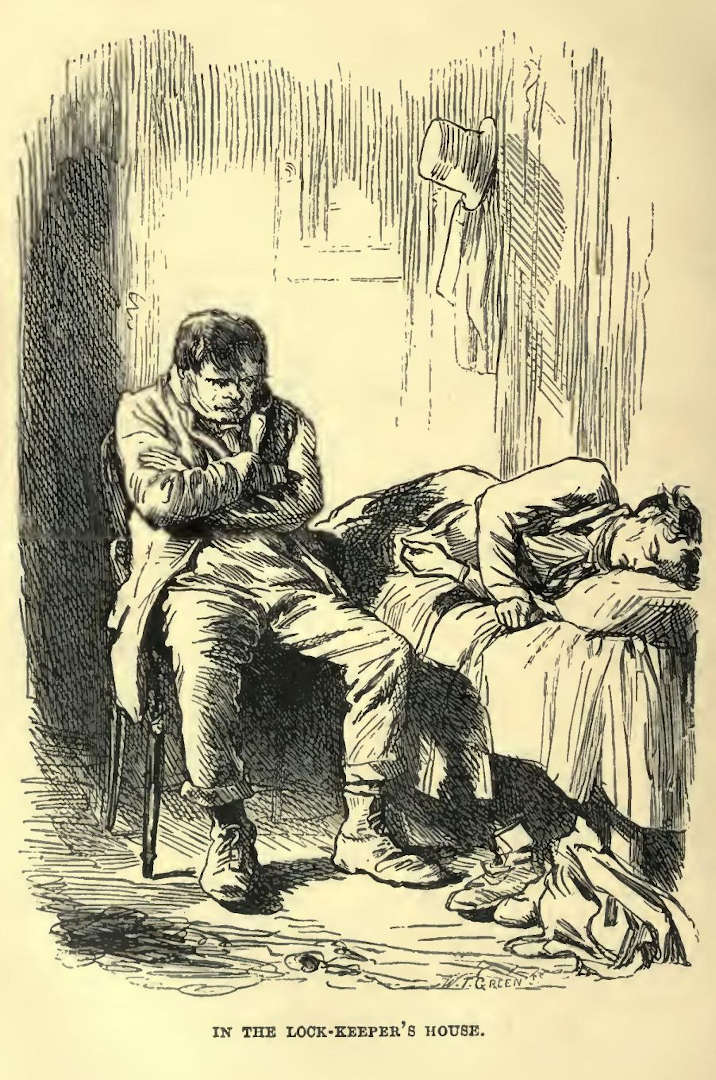
\includegraphics[scale=2.3]{04-01-01}

‘He sleeps sound,’ he said within himself; ‘yet he’s that up to me and
that noticing of me that my getting out of my chair may wake him, when a
rattling peal won’t; let alone my touching of him.’

He very cautiously rose to his feet. ‘T’otherest,’ he said, in a low,
calm voice, ‘are you a lying easy? There’s a chill in the air, governor.
Shall I put a coat over you?’

No answer.

‘That’s about what it is a’ready, you see,’ muttered Riderhood in a
lower and a different voice; ‘a coat over you, a coat over you!’

The sleeper moving an arm, he sat down again in his chair, and feigned
to watch the storm from the window. It was a grand spectacle, but not so
grand as to keep his eyes, for half a minute together, from stealing a
look at the man upon the bed.

It was at the concealed throat of the sleeper that Riderhood so often
looked so curiously, until the sleep seemed to deepen into the stupor
of the dead-tired in mind and body. Then, Riderhood came from the window
cautiously, and stood by the bed.

‘Poor man!’ he murmured in a low tone, with a crafty face, and a very
watchful eye and ready foot, lest he should start up; ‘this here coat
of his must make him uneasy in his sleep. Shall I loosen it for him,
and make him more comfortable? Ah! I think I ought to do it, poor man. I
think I will.’

He touched the first button with a very cautious hand, and a step
backward. But, the sleeper remaining in profound unconsciousness, he
touched the other buttons with a more assured hand, and perhaps the more
lightly on that account. Softly and slowly, he opened the coat and drew
it back.

The draggling ends of a bright-red neckerchief were then disclosed, and
he had even been at the pains of dipping parts of it in some liquid,
to give it the appearance of having become stained by wear. With a
much-perplexed face, Riderhood looked from it to the sleeper, and from
the sleeper to it, and finally crept back to his chair, and there, with
his hand to his chin, sat long in a brown study, looking at both.



